% Chapter Chapter 5 For Reproducible Research in R and RStudio
% Christopher Gandrud
% Created: 16/07/2012 05:45:03 pm CEST
% Updated: 13 October 2012




\chapter{Storing, Collaborating, Accessing Files, Versioning}\label{Storing}

In addition to being well organized, your research files need to be accessible for other researchers to be able to reproduce your findings. A useful way to make your files accessible is to store them on a cloud storage service\footnote{These services store your data on remote servers} \cite[see][]{Howe2012}. This chapter describes in detail two different cloud storage services--Dropbox and GitHub--that you can use to make your research files easily accessible to others. Not only do these services enable others to reproduce your research, they also have a number of benefits for your research workflow. Researchers often face a number of data management issues that, beyond making their research difficult to reproduce, can make doing the initial research difficult.

First, there is the problem of \textbf{storing} the data so that it is protected against computer failure--virus infections, spilling coffee on your laptop, and so on. Storing data locally--on your computer--or on a flash drive is generally more prone to loss than on remote servers in the cloud.

Second, we may work on a project with different computers and other devices. For example, we may use a computer at work to run computationally intensive analysis, while editing our presentation document on an tablet computer while riding the train to the office. So, we need to be able to \textbf{access} our files from multiple devices while in different locations. We often need a way for our \textbf{collaborators} to access and edit research files as well.

Finally, we almost never create a data set or write a paper perfectly all at once. We may make changes and then realize that we liked an earlier version, or parts of an earlier version better. This is a particularly important issue in data management where we may transform our data in unintended ways and want to go back to earlier versions. Also, when working on a collaborative project, one of the authors may accidentally delete something in a file that another author needed. To deal with these issues we need to store our data in a system that has \textbf{version control}. Version control systems keep track of changes we make to our files and allows us to access previous versions if we want to.

You can solve all of these problems in a couple of different ways using free or low cost cloud-based storage formats. In this chapter we will learn how to use Dropbox and GitHub for research file:

\begin{itemize}
    \item storage,
    \item accessing,
    \item collaboration,
    \item version control.
\end{itemize}

\section{Saving data in reproducible formats}

Before getting into the details of cloud-based data storage for all of our research files, lets consider what type of formats you should actually save your data in\index{data file formats}. A key issue for reproducibility is that others be able to not only get ahold of the exact data you used in your analysis, but be able to understand and use the data now and in the future. Some file formats make this easier than others.

In general, for small to moderately-sized data sets\footnote{I don't cover methods for storing and handling very large data sets--with high hundreds of thousands and more observations. For information on large data and R, not just storage, one place to look is this blog post by from RDataMining: \url{http://rdatamining.wordpress.com/2012/05/06/online-resources-for-handling-big-data-and-parallel-computing-in-r/} (posted 6 May 2012). One popular service for large file storage is Amazon S3\index{Amazon S3} (\url{http://aws.amazon.com/s3/}). I haven't used this service and can't suggest ways to integreate it with R.} a plain-text format like comma-separated values\index{comma-separated values} (\texttt{.csv}) or tab-separated values\index{tab-separated values}\footnote{Sometimes this format is called tab-delimited values\index{tab-delimited values}.} (\texttt{.tsv}) can be a good way to store your data. These formats simply store a data set as a text file. A row in the data set is a line in the text file. Data is separated into columns with commas or tabs, respectively. These formats are not dependent on a specific program. Any program that can open text files can open them including a wide variety of statistical programs other than R. This helps future proof your research. Version control systems that track changes to text, like GitHub--are also very effective version control systems with these types of files. 

To save data in a plain-text format with R use the \texttt{write.table} command\index{write.table}. For example, to save a data frame called {\emph{Data}} as a CSV file called {\emph{MainData.csv}} in our example {\emph{DataFiles}} directory (see Figure \ref{ExampleTree}):

\begin{knitrout}
\definecolor{shadecolor}{rgb}{0.969, 0.969, 0.969}\color{fgcolor}\begin{kframe}
\begin{alltt}
\hlfunctioncall{write.table}(Data, \hlstring{"/ExampleProject/Data/DataFiles/MainData.csv"},
                 sep = \hlstring{","})
\end{alltt}
\end{kframe}
\end{knitrout}


\noindent The \texttt{sep = ","} argument specifies that we want to use a comma to separate the values. For CSV files you can use a modified version of this command called \texttt{write.csv}\index{write.csv}. This command simply makes it so that you don't have to write \texttt{sep = ","}. 

If you want to save your data with rows separated by tabs, rather than commas, simply set the argument \texttt{sep = "\textbackslash{}t"} and the file extension to \texttt{.tsv}.\label{TSVEscape}

R is also able to save data in a wide variety of other file formats, mostly through the {\emph{foreign}} package (see Chapter \ref{DataGather}). These formats may be less future proof than simple text-formatted data files.

\section{Storing your files in the cloud}

In this book we'll cover two (largely) free cloud storage services that allow you to store, access, collaborate on, and version control your research files. These services are Dropbox and GitHub.\footnote{Dropbox provides a minimum amount of storage for free, above which they charge a fee. GitHub lets you create publicly accessible repositories--kind of like project folders--for free, but they charge for private repositories.} Though they both meet our basic storage needs, they do so in different ways and require different levels of effort to set up and maintain.

These two services are certainly not the only way to make your research files available. Research oriented services include the SDSC Cloud,\footnote{\url{https://cloud.sdsc.edu/hp/index.php}} the Dataverse Network Project,\footnote{\url{http://thedata.org/}}, figshare\footnote{\url{http://figshare.com/}} and RunMyCode.\footnote{\url{http://www.runmycode.org/}} These services include good built-in citation systems, unlike Dropbox and GitHub. They may be a very good place to store research files once the research is completed or close to completion. Some journals are beginning to require key reproducibility files be uploaded to these sites. However, these sites' ability to store, access, collaborate on, and version control files \emph{during} the main part of the research process is mixed. Services like Dropbox and Github are very capable of being part of the research workflow from the beginning.

\subsection{Dropbox}

The easiest types of cloud storage for your research are services like Dropbox\footnote{\url{http://www.dropbox.com/}} and Google  Drive.\footnote{\url{https://drive.google.com/}} These services not only store your data in the cloud, but also provide some way to share files and even includes basic version control capabilities. I'm going to focus on Dropbox because it currently offers a complete set of features that allow you to store, version, collaborate, and access your data. I will focus on how to use Dropbox on your computer. Some Dropbox functionality may be different on mobile devices.

\subsection{Storage}

When you sign up for Dropbox and install the program\footnote{See \url{https://www.dropbox.com/downloading} for downloading and installation instructions.} it creates a directory on your computer's hard drive. When you place new files and folders in this directory and make changes to them, Dropbox automatically syncs the directory with a similar folder on a cloud-based server. Typically you can sign up to the service and receive a limited amount of storage space for free; usually a few gigabytes.

\subsubsection{Accessing Data}

There are two similar, but importantly different ways to access data stored on Dropbox. All files stored on Dropbox have a URL address through which they can be accessed from a computer connected to the internet. Some of these files can be easily loaded directly into R, while others must me manually (point-and-click) downloaded onto your computer and then loaded into R. Files in the \emph{Public}\index{Dropbox Public folder} folder can be downloaded directly into R. Files not in the \emph{Public} folder have to be downloaded  manually.\footnote{This is not completely true. It could be possible to create a web scraper\footnote{web scraper} that could download data from a file not in your \emph{Public} folder. However, this is kind of a hassle and not practical, especially since the accessing files from the \emph{Public} folder is so easy.}

Either way you find a file's URL address by first right-clicking on the file icon in you Dropbox folder. If the file is stored in the \emph{Public} folder, you go to \texttt{Dropbox} in the menu that pops up, then click \emph{Copy Public Link}. This copies the URL into your clipboard from where you can paste it into your R source code (or wherever). Once you have the URL you can load the file directly into R using the \texttt{read.table} command for data frames (see Chapter 5) or the \texttt{source} command for source code files (see Chapter 8).

To give you a preview of how to download data directly into R from Dropbox, try downloading a data file from my Public folder. The full URL of the data set is: \url{http://dl.dropbox.com/u/12581470/code/Replicability_code/Fin_Trans_Replication_Journal/Data/public.fin.msm.model.csv}. I've used the URL shortening service bitly\footnote{See \url{https://bitly.com/}.}
to make this link fit on the page.

\begin{knitrout}
\definecolor{shadecolor}{rgb}{0.969, 0.969, 0.969}\color{fgcolor}\begin{kframe}
\begin{alltt}
\hlcomment{# Download data stored in a Dropbox Public folder}
\hlcomment{# and save as an object named Data}
Data <- \hlfunctioncall{read.table}(\hlstring{"http://bit.ly/PhjaPM"}, 
                    sep = \hlstring{","}, header = TRUE)
                    
\hlcomment{# Show variables in Data}
\hlfunctioncall{names}(Data)
\end{alltt}
\begin{verbatim}
## [1] "idn"        "country"    "year"       "reg_4state"
\end{verbatim}
\end{kframe}
\end{knitrout}


If the file is not in your \emph{Public} folder you also go to \texttt{Dropbox} after right-clicking on the file. Then choose \texttt{Get Link}. This will open a webpage in your default web browser from where you can download the file. You can copy and paste the page's URL from your browser's address bar. You can also get these URL links through the online version of your Dropbox. First log into the Dropbox website. If the file is in your \emph{Public} folder, right-click on it and then select \texttt{Copy Public Link}. When you hover your curser over a file or folder not in the \emph{Public} Folder you will see a chain-link icon appear on the far right. Clicking on this icon will get you the link.

Storing files in the \emph{Public} folder clearly makes replication easier because the files can be downloaded and run directly in R.

\subsection{Collaboration}

Though others can easily access your data and files through Dropbox URL links, you cannot save files through the link. You must save files in the Dropbox folder on your computer or upload them through the website. If you would like collaborators to be able to modify the research files you will need to `share' the Dropbox folder with them. You cannot share your \emph{Public} folder, so you will need to keep the files you want collaborators to be able to modify in a non-public folder. Once you create this folder you can share it with your collaborators by right-clicking on the folder and selecting \texttt{Invite to folder} on the Dropbox website or \texttt{Dropbox} \textrightarrow\: \texttt{Share This Folder\ldots} on the locally stored folder. Enter your collaborator's email address when prompted. They will be sent an email that will allow them to accept the share request and, if they don't already have an account, sign up for Dropbox.

\subsubsection{Version control}

Dropbox has a simple version control system. Every time you save a document on Dropbox a new version is created. To view a previous version, navigate to the file on the Dropbox website. Then right-click on the file. In the menu that pops up select \texttt{Previous Versions}. This will take you to a webpage listing previous versions of the file, who created the version, and when it was created. A new version of a file is created every time you save a file and it is synced to the Dropbox cloud service. 

\subsection{GitHub}

Dropbox adequately meets our four basic criteria for reproducible data storage and is easy to set up. GitHub meets the criteria and more, but is less straightforward at first.

GitHub is an interface and cloud hosting service built on top of the Git\index{Git} version control system. GitHub was not explicitly designed to host research projects or even data. It was designed to host ``socially coded" computer programs--in what Git calls ``repositories"\index{repository}--by making it easy for a number of collaborators to work together to build computer programs. This seems very far from reproducible research.

Remember that as reproducible researchers we are building projects out of interconnected text files. In important ways this is exactly the same as building a computer program. Computer programs are also basically large collections of interconnected text files. Like computer programers, we need ways to store, version control, access, and collaborate on our text files. Because GitHub is very actively used by people with very similar needs (who are also really good programmers), the interface offers many highly developed and robust features for reproducible researchers.

GitHub's extensive features and heart in the computer programming community means that it takes a longer time than Dropbox to set it up and become familiar with it. So we need good reasons to want to invest the time needed to learn GitHub compared to Dropbox and similar services. Here is a list of GitHub's advantages over Dropbox for reproducible research that will hopefully convince you to get started using it: \\[0.25cm]

\noindent{\bf{Storage and Access}}
\begin{itemize}
    \item Dropbox simply creates folders stored in the cloud which you can share with other people. GitHub makes your projects accessible on a fully featured project website (see Figure \ref{BookRepository}). An example feature is that it automatically renders Markdown files called {\emph{README.md}}\footnote{You can use a variety of other markup languages as well. See \url{https://github.com/github/markup}.} in a GitHub directory on the repository's website. This makes it easy for independent researchers to find the file and read it.   
    \item Public repositories--those viewable by anyone--can be downloaded by anyone in a compressed format.
    \item GitHub can create and and host a website for your research project that you could use to present the results, not just the replication files.
\end{itemize} 

\vspace{0.25cm}
       
\noindent{\bf{Collaboration}} \\[0.25cm]

Dropbox allows multiple people to share files and change them. GitHub does this and more:

\begin{itemize}
        \item GitHub keeps meticulous records of who contributed what to a project.
        \item Each GitHub repository has an ``Issues'' area where you can note issues and discuss them with your collaborators. Basically this is an interactive to-do list for your research project. It also stores the issues so you have a full record.
        \item Each repository can also host a wiki\index{wiki} that, for example, could explain in detail how certain aspects of a research project were done.
        \item Anyone can suggest changes to files in a public repository. These changes can be accepted or declined by the project's authors. The changes are recorded by the Git version control system. This could be especially useful if an independent researcher notices an error. 
\end{itemize}

\vspace{0.25cm}

\begin{wrapfigure}{r}{0.5\textwidth}
    \caption{A Basic Git Repository with Hidden {\emph{.git}} Folder Revealed}
    \label{BasicGitRepo}
        \begin{center}    
        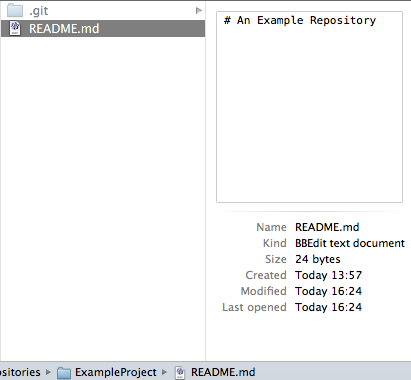
\includegraphics[width=0.45\textwidth]{/git_repositories/Rep-Res-Book/Source/Children/Chapter5/images5/BasicGitRepository.png}
        \end{center}
\end{wrapfigure}

\noindent{\bf{Version Control}}    
\begin{itemize}
\item
  Dropbox's version control system only lets you the see files' names, the times they were created, who created them, and revert back to specific versions. Git tracks every change you make. The GitHub website and GUI programs for Mac and Windows provide nice interfaces for examining specific changes in text files.
\item
  Dropbox creates a new version every time you save a file. This can make it difficult to actually find the version you want as the versions quickly multiply. Git's version control system only creates a new version when you tell it to.
\item
  Dropbox does not merge conflicting versions of a file together. This can be annoying when you are collaborating on project and more than one author is making changes to documents at the same time. GitHub identifies conflicts and lets you reconcile them.
\item
  Git is directly integrated into RStudio Projects\index{RStudio Projects}.\footnote{RStudio also supports the Subversion version
  control system, but I don't cover that here.}
\end{itemize}

\subsubsection{Setting up GitHub: Basic}

There are two ways to set up and use GitHub on your computer. You can use the command line version of Git. It's available for Mac and Linux (in the Terminal\index{Terminal}) as well as Windows (through Git Bash\index{Git Bash}).\footnote{The interface for Git Bash looks a lot like the Terminal or Windows PowerShell. On Windows computers you need it to run Git.} You can also use the Graphical User Interface GitHub program. Currently it's only available for Windows and Mac. Installing the GUI version of GitHub also installs Git. The GitHub website has excellent step-by-step instructions for how to install both versions. 

The first thing to do to setup GitHub is go to their website (\url{https://github.com/}) and sign up for an account. Second, you should go to the following website for instructions on setting up Git: \url{https://help.github.com/articles/set-up-git}. The instructions on that website are very comprehensive, so I'll direct you there for the full setup information. 

\subsubsection{Storage on GitHub}

\paragraph{Setting up Git repositories locally}
After you set up your GitHub account you'll need to set up a Git repository\index{Git repository}. Git keeps track of changes made to any file in a repository. GitHub stores repositories remotely. Repositories are kind of like folders, it's probably best to think of them as your projects' parent directories.

You can setup a Git repository on your computer with the command line.\footnote{Much of the discussion of the command line in this section is inspired by Nick Farina's blog post on Git (see \url{http://nfarina.com/post/9868516270/git-is-simpler}, accessed 24 November 2012).} I keep my repositories in a folder called {\emph{git\_repositories}}.\footnote{To follow along with this code you will first need to create a folder called {\emph{git\_repositories}} in your root directory.} It has the root folder as its parent. Imagine that we want to set up a repository in this directory for a project called {\emph{ExampleProject}}. Initially it will have one README file called {\emph{README.md}}. To do this we would first type into the Terminal for Mac and Linux computers:

\begin{knitrout}
\definecolor{shadecolor}{rgb}{0.969, 0.969, 0.969}\color{fgcolor}\begin{kframe}
\begin{verbatim}
# Make new directory 'ExampleProject
mkdir /git_repositories/ExampleProject

# Change to directory 'ExampleProject'
cd /git_repositories/ExampleProject

# Create new file README.md
echo "# An Example Repository" > README.md
\end{verbatim}
\end{kframe}
\end{knitrout}


\noindent So far we have only made the new directory and set it as our working directory (see Chapter \ref{DirectoriesChapter}). Then with the \texttt{echo} Shell command we created a new file named {\emph{README.md}} that includes the text ``\# An Example Repository". Note that the code is basically the same in Windows PowerShell, though obviously the directory names are different. Also, you don't have to do these steps in the command line. You could just created the new folders and files the same what that you normally do with your mouse.

Now we can tell git that the we want to treat the directory {\emph{ExamplProject}} as a repository and that we want to track changes made to the file {\emph{README.md}}. Use Git's \texttt{init} (initialize) command to set up directory as a repository. See Table \ref{GitCommandsTable} for the list of Git commands covered in this chapter.\footnote{For a comprehensive guide to Git commands see \url{http://git-scm.com/}.} Use Git's \texttt{add} command to add a file to the Git repository. For example, 

\begin{knitrout}
\definecolor{shadecolor}{rgb}{0.969, 0.969, 0.969}\color{fgcolor}\begin{kframe}
\begin{verbatim}
# Initialize the Git repository
git init

# Add README to the repository
git add README.md
\end{verbatim}
\end{kframe}
\end{knitrout}


\noindent You probably noticed that you always need to put \texttt{git} before the command. This tells the command line what program the command is from. When you initialize a folder as a Git repository a hidden folder called {\emph{.git}} is added to the directory (see Figure \ref{BasicGitRepo}). This is where all of your changes are kept. If you want to add all of the files in the working directory to the Git repository type:

\begin{knitrout}
\definecolor{shadecolor}{rgb}{0.969, 0.969, 0.969}\color{fgcolor}\begin{kframe}
\begin{verbatim}
# Add all files to the repository
git add .
\end{verbatim}
\end{kframe}
\end{knitrout}


\noindent Now when we want Git to track changes made to files added to the repository we can use the \texttt{commit}\index{git commit} command. In Git language we are ``committing" the changes to the repository.

\begin{knitrout}
\definecolor{shadecolor}{rgb}{0.969, 0.969, 0.969}\color{fgcolor}\begin{kframe}
\begin{verbatim}
# Commit changes
git commit -a -m "First Commit, created README file"
\end{verbatim}
\end{kframe}
\end{knitrout}


\nodindent The \texttt{-a} (all) command commits changes to all of the files that have been added to the repository. You can include a message with the commit using the \texttt{-m} command like: \texttt{"First Commit, created README file"} Messages help you remember general details of the individual commit. This is helpful when you want to revert to old versions.

\noindent \textbf{Remember:} Git only tracks changes when you commit them. 

Finally, you can use the \texttt{status} command for details about your repository, including un committed changes. Generally it's a good idea to use the \texttt{-s} (short) argument, so that the output is more readable.

\begin{knitrout}
\definecolor{shadecolor}{rgb}{0.969, 0.969, 0.969}\color{fgcolor}\begin{kframe}
\begin{verbatim}
# Display status
git status -s
\end{verbatim}
\end{kframe}
\end{knitrout}


\begin{table}
  \caption{A Selection of Git Commands}
  \begin{center}
  \label{GitCommandsTable}
  \begin{tabular}{l p{5cm}}
    \hline  
    Command & Description \\[0.25cm] \hline\hline
    \texttt{init} & Initialize a Git repository. \\[0.25cm]
    \texttt{add} & Add a file to a Git repository. \\[0.25cm]
    \texttt{commit} & Commit changes to a Git repository. \\[0.25cm]
    \texttt{status} & Show the status of a Git repository including uncommitted changes made to files. \\[0.25cm]
    \texttt{checkout} & Checkout a branch. \\[0.25cm]
    \hline
  \end{tabular}
  \end{center}
\end{table}

Before discussion how to host a Git repository on GitHub it is useful to step back for a second and try to understand what Git is doing when you commit your changes. In the hidden {\emph{.git}} folder Git is saving all of the information in compressed form from each of your commits into a subfolder called {\emph{Objects}}. Commit objects\index{Git commit object}\footnote{Other Git objects include trees (sort of like directories) and blobs (individual files).} are everything from a particular commit. I mean everything. If you delete all of the files in your repository (except for the {\emph{.git}} folder) you can completely recover all of the files from your most recent commit with the \texttt{checkout} command:

\begin{knitrout}
\definecolor{shadecolor}{rgb}{0.969, 0.969, 0.969}\color{fgcolor}\begin{kframe}
\begin{verbatim}
# Checkout latest commit
git checkout --
\end{verbatim}
\end{kframe}
\end{knitrout}


\noindent We'll look at the \texttt{checkout} command in more detail later. 

\paragraph{Setting up GitHub remote repositories}

\begin{figure}[t]
    \caption{Part of this Book's GitHub Repository Webpage}
    \label{BookRepository}
    \begin{center}
    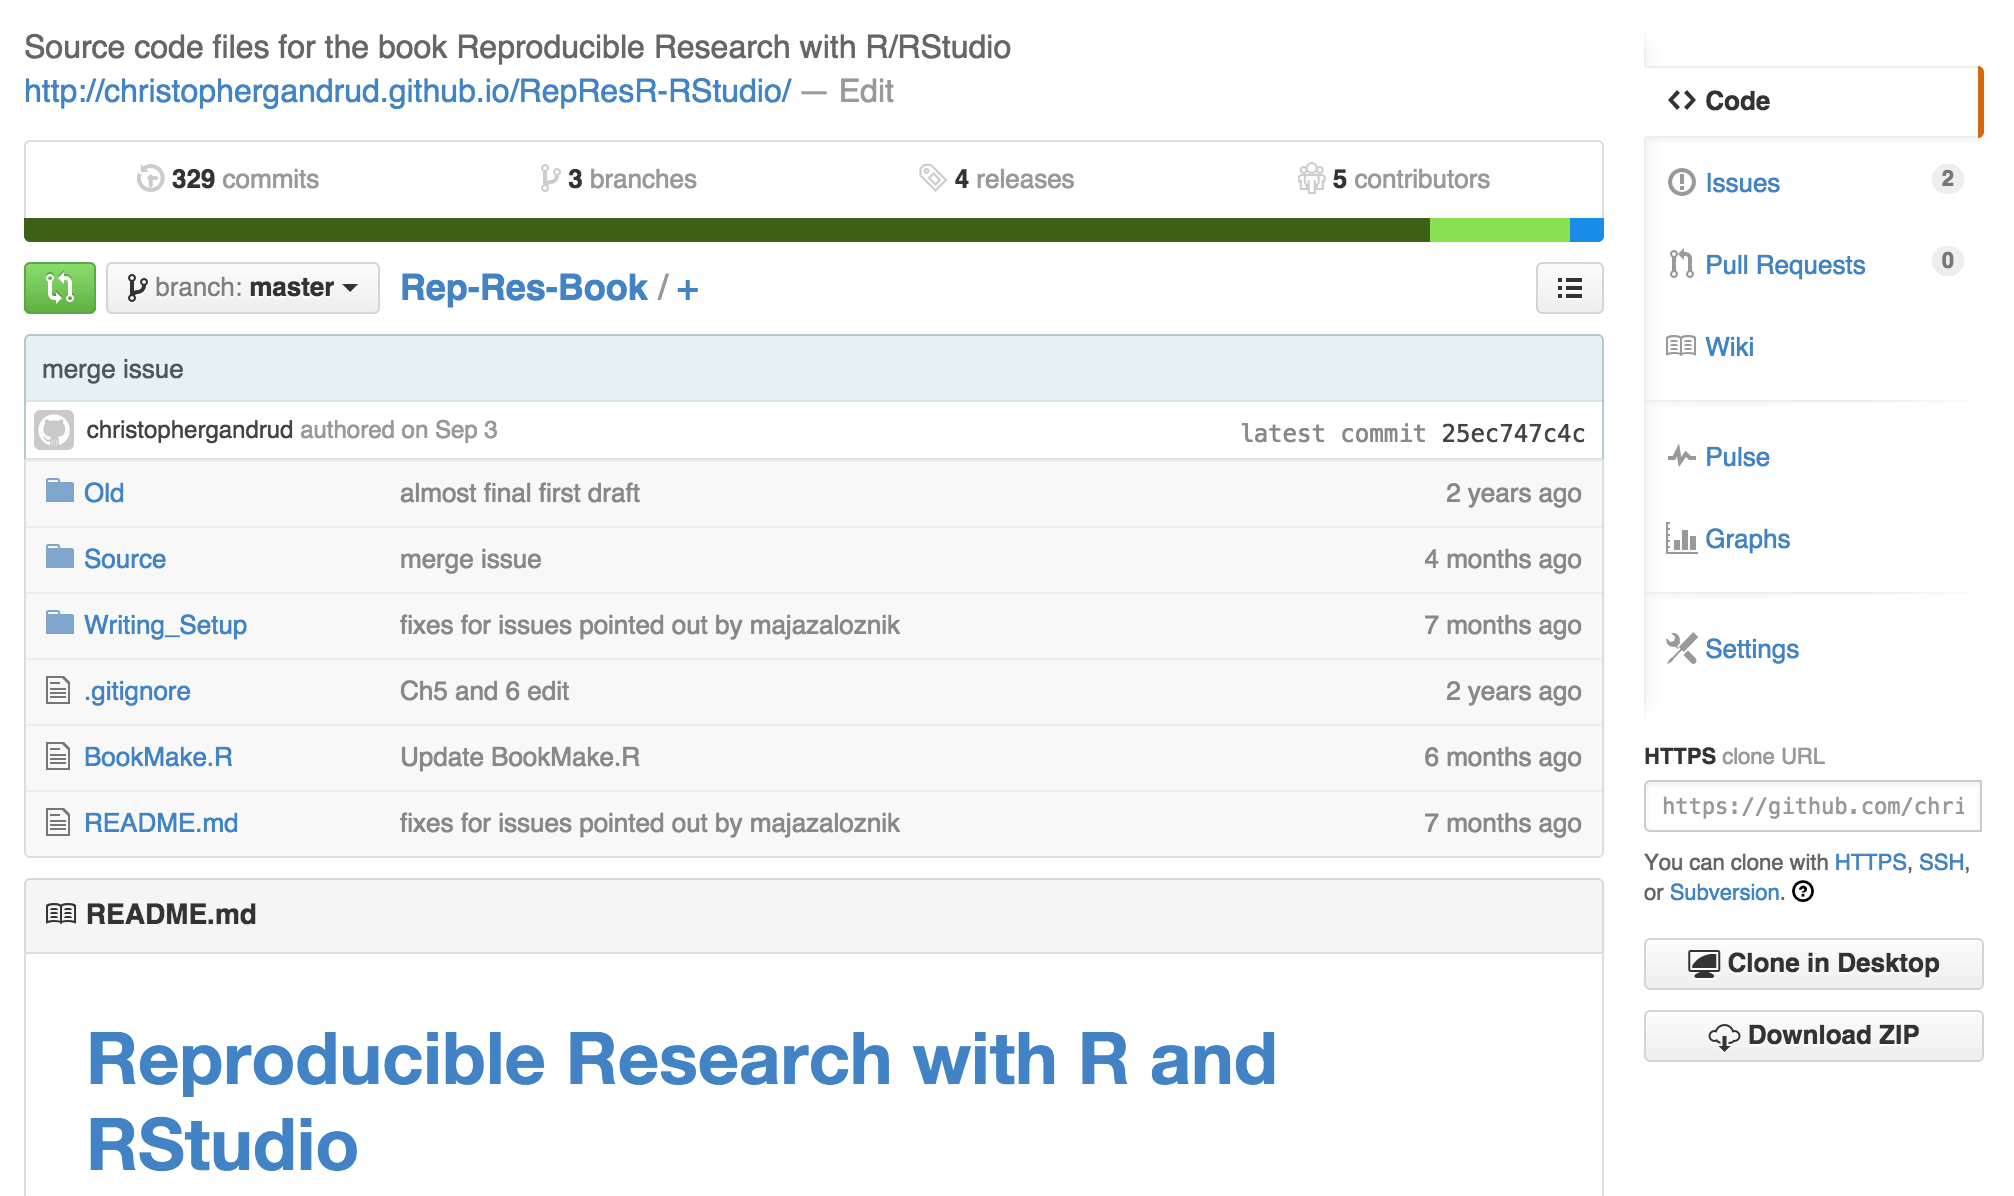
\includegraphics[scale=0.5]{/git_repositories/Rep-Res-Book/Source/Children/Chapter5/images5/GitHubReadme.png}
    \end{center}
\end{figure}

\paragraph{Setting up GitHub with RStudio Projects}

Once you have your repository set up on GitHub you can clone it onto your computer and create an RStudio Project\index{RStudio Projects}

\subsubsection{Accessing on GitHub}

\subsubsection{Collaboration with GitHub}

Repositories can have official collaborators. Public repositories can have unlimited collaborators. Anyone with a GitHub account can be a collaborator. 
 

Anyone with a GitHub account can make changes to files in a public repository on the repository's website. Simply click the \texttt{Edit} button above the file and make edits. If the person making the edits is not a repository collaborator, their edit will be sent to the repository's owner for approval.\footnote{This is called a \texttt{pull}\index{git pull} in git terminology}. This is a useful way for independent researchers to catch errors and directly address them.

\paragraph{Branches}

\paragraph{Syncing repository}

\subsubsection{Version Control with GitHub}

GitHub's version control system is much more comprehensive than Dropbox's. However, it also has a steeper learning curve.

\paragraph{Reverting to an old version of a file}

You can use the {\tt{git checkout}} command to revert to a previous version of a document, because you accidentally deleted something important or made other changes you don't like. To `checkout' a particular version of a file type:

\begin{knitrout}
\definecolor{shadecolor}{rgb}{0.969, 0.969, 0.969}\color{fgcolor}\begin{kframe}
\begin{alltt}
git checkout COMMITREF FILENAME
\end{alltt}
\end{kframe}
\end{knitrout}


\noindent Now the previous version of the file is in your working directory, where you can commit it as usual.

Let's break down the code.  {\tt{FILENAME}} is the name of the file that you want to change\footnote{If it is in a repository's subdirectory you will need to include this in the file name.} and {\tt{COMMITREF}} is the reference that git gave to the commit you want to revert back to. The reference is easy to find and copy in GitHub. On the file's GitHub page click on the {\tt{History}} button. This will show you all of the commits. By clicking on {\tt{Browse Code}} you can see what the file at that commit looks like. Above this button is another with a series of numbers and letters. This is the commit's SHA (Secure Hash Algorithm)\index{SHA}. For our purposes, it is the commit's reference number. Click on the {\tt{Copy SHA}} button to the left of the SHA to copy it. You can then paste it as an argument to your {\tt{git checkout}} command. 

\paragraph{More Practice with Command Line Git \& GitHub}

If you want more practice setting up GitHub in the command line, GitHub and the website Code School have an interactive tutorial that you might find interesting. You can find it at: \url{http://try.github.com/levels/1/challenges/4}.
